\def\vector#1{\mbox{\boldmath $#1$}}

\begin{figure*}[htbp]
 \begin{center}
  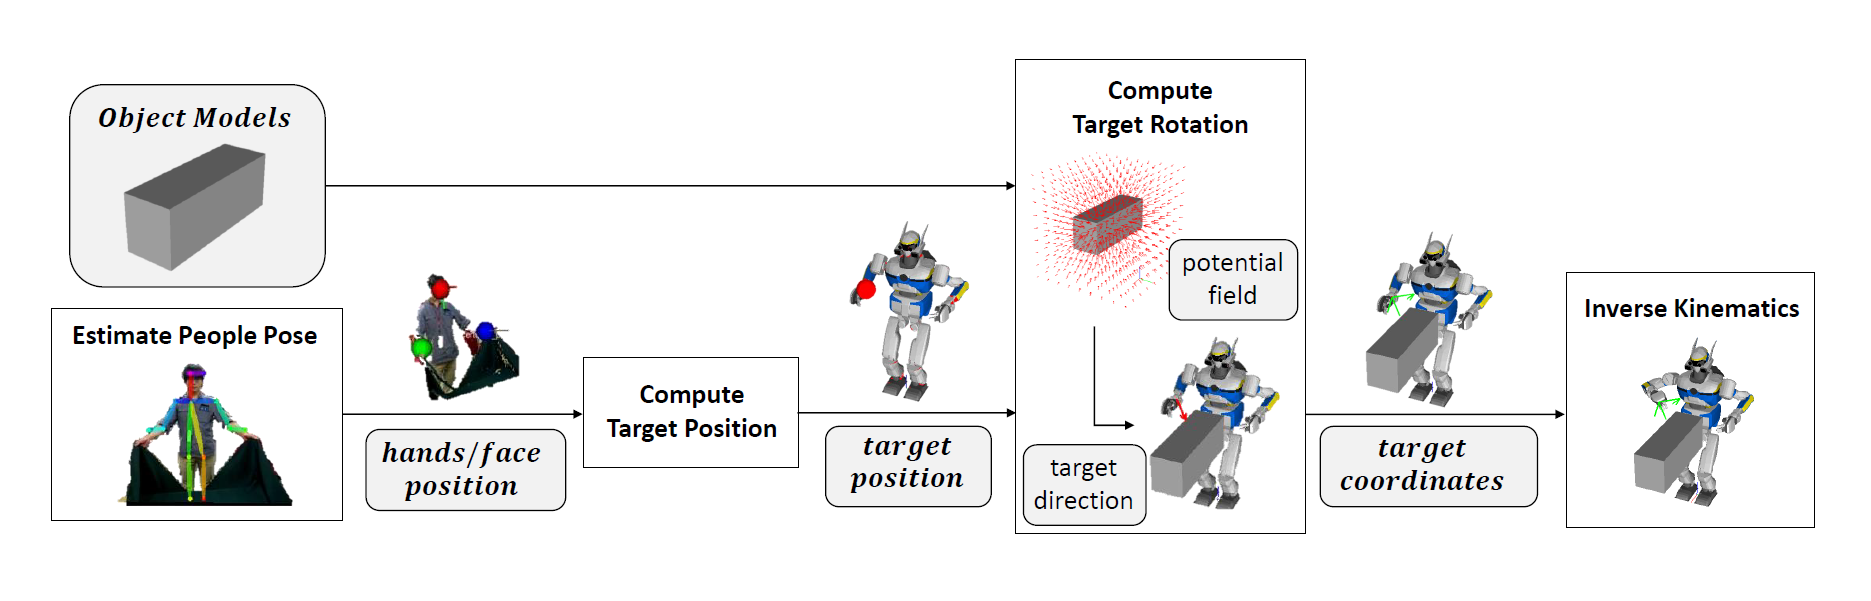
\includegraphics[width=1.80\columnwidth]{figs/flow_en.png}
  \vspace{-3mm}
  \caption{Overall flow of decision in robot arm motion}
  \label{figure:flow}
 \end{center}
 \vspace{-6mm}
\end{figure*}

\section{Acquiring Robot Autonomous Arm Motions}
\label{sec:motion_generator}
\figref{flow} shows our proposed flow of deciding robot arm motion in cooperative-operation tasks. In this section, first, we will describe the method to acquire the target positions of the robot hands by means of imitation, considering the positions of human hands and face acquired by applying OpenPose~\cite{OpenPose} (\subsecref{position}).
Second, we will describe the idea to acquire the target orientation of the robot hands with the consideration of the potential vector field of environmental objects (\subsecref{orientation}).

\subsection{Acquiring Target Positions of Robot Hands}
\label{subsec:position}
In situations of cooperative works where a human and a robot manipulate the same object at the same time with facing each other, the target coordinates of the robot hands can be decided by observing human hand motions and imitating them symmetry. Since the acquired three dimensional positions of the human hands are relative to the robot camera, those have to be translated as those relative to the human. Positions of the human hands relative to the human face that are described in the human coordinate system \(^{f}\!\vector{p}^{hmn}_{rh}\), \(^{f}\!\vector{p}^{hmn}_{lh}\) are calculated as below.

\vspace{-3mm}
\begin{align}
^{f}\!\vector{p}^{hmn}_{rh} &= (\bm{R}^{hum}_{f})^{T}(\vector{p}^{hmn}_{rh} - \vector{p}^{hmn}_{f})\\
^{f}\!\vector{p}^{hmn}_{lh} &= (\bm{R}^{hum}_{f})^{T}(\vector{p}^{hmn}_{lh} - \vector{p}^{hmn}_{f})
\end{align}

\(\vector{p}^{hmn}_{f}\), \(\vector{p}^{hmn}_{rh}\), \(\vector{p}^{hmn}_{lh}\) refer to the position of the human face and hands relative to the world coordinate system. \(\bm{R}^{hum}_{f}\) refers to a rotation matrix from the world coordinate system to the human coordinate system, which is set at the position of the human face. This is predetermined as a constant matrix below according to the angle between the human and the robot.

\vspace{-3mm}
\begin{equation}
  \bm{R}^{hum}_{f} = \bm{R}_z(\theta)
  =
  \left(
  \begin{array}{rrr}
    \cos{\theta} & \sin{\theta} & 0\\
    -\sin{\theta} & \cos{\theta} & 0\\
    0 &            0 & 1\\
  \end{array}
  \right)
\end{equation}

The target positions of the robot right and left hands are decided by referring to the human left and right hand respectively. Target positions of the robot hands relative to the robot face that are described in the robot coordinate system \(^{f}\!\vector{p}^{rbt}_{rh}\),\(^{f}\!\vector{p}^{rbt}_{lh}\) can be acquired as below.

\vspace{-3mm}
\begin{eqnarray}
  ^{f}\!\vector{p}^{rbt}_{rh} &=& \bm{A} \ \ ^{f}\!\vector{p}^{hmn}_{lh}\\
  ^{f}\!\vector{p}^{rbt}_{lh} &=& \bm{A} \ \ ^{f}\!\vector{p}^{hmn}_{rh}\\
  where \ \ \bm{A} &=&
  \left(
  \begin{array}{rrr}
    1 &  0 & 0\\
    0 & -1 & 0\\
    0 &  0 & 1\\
  \end{array}
  \right) \nonumber
  \label{equation:robot_hand_pos_ref_robot_face}
\end{eqnarray}

Finally, after translating these acquired target hand positions as those defined in the world coordinate system, the target positions of the robot hands \(\vector{p}^{rbt}_{rh}\), \(\vector{p}^{rbt}_{lh}\), can be acquired, which are the symmetrical imitation of the human hands.

\vspace{-3mm}
\begin{eqnarray}
  \vector{p}^{rbt}_{rh} &=& \bm{R}^{rbt}_{f} \ \ ^{f}\!\vector{p}^{rbt}_{rh} + \vector{p}^{rbt}_{f}\\
  \vector{p}^{rbt}_{lh} &=& \bm{R}^{rbt}_{f} \ \ ^{f}\!\vector{p}^{rbt}_{lh} + \vector{p}^{rbt}_{f}
  \label{equation:robot_hand_pos}
\end{eqnarray}

\(\vector{p}^{rbt}_{f}\) refers to the position of the robot head and \(\bm{R}^{rbt}_{f}\) to a rotation matrix from the world coordinate system to the robot face coordinate system, which are predetermined constant vector and matrix.\(\bm{R}^{rbt}_{f}\) is basically equal to the identity matrix \(\bm{E}\); the orientations of the robot face coordinate system and the world coordinate system are the same.

\subsection{Acquiring Target Orientations of Robot Hands}
\label{subsec:orientation}

%% \vspace{-3mm}
\begin{figure}[htbp]
 \begin{center}
  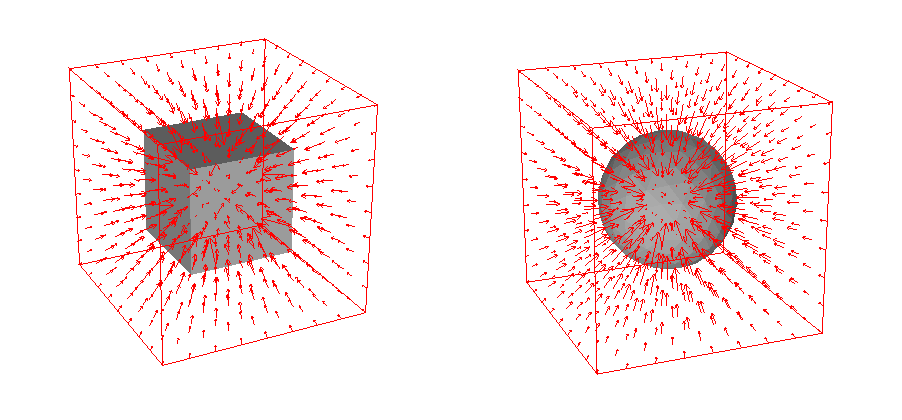
\includegraphics[width=0.70\columnwidth]{figs/electronic-potential-cube-sphere.png}
  \vspace{-3mm}
  \caption{Examples of vector fields of a cube and a sphere}
  \label{figure:electronic_potential}
 \end{center}
 %% \vspace{-3mm}
\end{figure}

Generally, it is hard to recognize the human hand orientation only by a two dimensional image. In order to decide the target orientations of the robot hands, we introduce the idea of potential method.
Providing the geometry of the object is known, we introduce the vector field whose direction faces toward or against the object surface. The target orientation is determined as a posture such that the palm is oriented in that direction. The vector \(\vector{E}(\vector{r})\) driven by the potential field of the object at a position \(\vector{r}\) is calculated as following.

\vspace{-3mm}
\begin{equation}
  \label{equation:electronic_potential}
  \vector{E}(\vector{r}) = - \sum_{A' \in A}{ \int_{A'} \frac {\sigma (\vector{r'})} {\| \vector{r} - \vector{r'} \| ^ 2} \cdot \frac {\vector{r} - \vector{r'}} {\| \vector{r} - \vector{r'} \|} dA' }
\end{equation}

\(A\) refers to the set of the object surfaces, and \(\vector{r'}\) to points on the surface \(A' (\in A)\).\(\sigma (\vector{r'})\) refers to the surface density of a virtual chage at the position \(\vector{r'}\), that is, the strength of attraction or repulsion. In this research, this value is set to be constant and to satisfy \(|\sigma (\vector{r'})| = 1\). Note that changing the sign of \(\sigma (\vector{r'})\), the potential field can be switched between attraction and repulsion.\par
While \equref{electronic_potential} includes an area fraction, it has to be discretized when simulating. It is done by dividing each surface into small meshes along one set of two adjacent edges and supposing a charge on each meshgrid. Below shows the discretized equation of \equref{electronic_potential}.

\vspace{-3mm}
\begin{equation}
  \label{equation:electronic_potential_simple}
  \vector{E}(\vector{r}) = - \sum_{A' \in A} {\sum_{\vector{p} \in MG(A')} { \frac {\sigma'} {\| \vector{r} - \vector{r'}(\vector{p}) \| ^ 2} \cdot \frac {\vector{r} - \vector{r'}(\vector{p})} {\| \vector{r} - \vector{r'}(\vector{p}) \|} } }
\end{equation}

Here, \(MG(A')\) is the set of meshgrids of surface \(A'\).
\figref{electronic_potential} describes the example of vector fields generated by \equref{electronic_potential_simple} on a cube and a sphere.\par
The target coordinate of the robot hand is acquired as a posture such that the palm is oriented in the direction at the target position acquired in \subsecref{position}.
